
Le informazioni saranno raccolte tramite intervista, e allegheremo del materiale informativo preso da quanto si trova di pubblico di un gioco di ruolo Online.\\
Dopo svariati tentativi falliti di contattare via email delle persone che lavorano su WOW abbiamo contattato, 
tramite amici di amici dei giovani programmatori e ingegneri che stanno sviluppando la loro idea di Mmorpg e sono stati disponibili ad aiutarci.


%------------------------------------------------
\subsubsection{Prima Intervista - Game Director} % Sotto_Sotto-Sezione

\medskip

%Per le Interviste questo metodo è ottimo:
%\begin{description}[style=nextline]
%\item[DOMANDA]RISPOSTA  Fare attenzione alle lettere accentate che potrebbero non essere riconosciute
%non scordare di mettere la chiusura di description alla fine   \end{description}

\begin{description}[style=nextline]
    \item[Ciao, sappiamo che hai esperienza nello sviluppo di giochi di ruolo online, potresti dirci innanzitutto di cosa si tratta?]Certo, proprio attualmente n\'{e} sto sviluppando uno ambientato in un mondo fantasy medievale. Dove ogni giocatore puo creare un suo alter ego ed iniziare la sua avventura, da solo oppure insieme ad altri giocatori. Lo scopo iniziale del gioco \'{e} quello di acquisire punti esperienza in maniera da salire di livello. In questo modo il personaggio creato diventa pi\'{u} forte, acquisendo maggiori punti vita e aumentando le sue Statistiche Base cio\'{e} forza,intelligenza e destrezza. Con l'aumento del livello si ha la possibilit\'{a} apprendere nuove abilit\'{a} e di indossare pezzi di equipaggiamento pi\'{u} potenti. Una volta raggiunto il livello massimo, di solito 100 l'obiettivo del giocatore \'{e} quello di ottenere pezzi di equipaggiamento migliori sconfiggendo mostri particolarmente forti chiamati boss
    
    \item[Cosa deve fare l'utente per iniziare a giocare?] Una volta scaricato e avviato il client di gioco l'utente si trova davanti alla schermata di login. Qui dovr\'{a} inserire le stesse credenziali utilizzate sul sito principale per effettuare l'accesso. Una volta dentro, se il giocatore ha gi\'{a} un personaggio pu\'{o} iniziare a giocare. Altrimenti deve fare la procedura di creazione dello stesso e iniziare il gioco. Se l'utente lo desidera, puo eliminare un personaggio gi\'{a} creato. 
     
    \item[In cosa consiste la creazione del personaggio?] Attraverso un interfaccia grafica l'utente deve scegliere un nome composto da sole lettere per il personaggio, la razza di appartenenza tra umano, elfo o nano, le sue caratteristiche fisiche come capelli, volto, barba, colore della pelle...Si definisce la classe di combattimento: guerriero, mago o arciere. La scelta delle classi di combattimento \`{e} legata alla razza di appartenenza ad eccezione dell'umano che pu\`{o} essere quello che vuole. L'elfo pu\`{o} essere un arciere oppure un mago mentre non esistono nani maghi.
    
	\item[In che modo incidono queste scelte all'interno del gioco?] Sono fattori puramente estetici, ad eccezione della classe di combattimento che va ad incidere sullo stile di combattimento del personaggio, quindi sulle abilit\`{a} che pu\`{o} apprendere. Inoltre ogni classe pu\`{o} utilizzare solo certi tipi di equipaggiamento. Il guerriero utilizza spade, asce, mazze e pu\`{o} indossare armature pesanti. Il mago utilizza bastoni,bacchette magiche e indossa armature leggere. L'arciere utilizza archi, balestre e indossa armature medie
	
	\item[Potresti illustrare in poche parole le meccaniche del gioco?] Una volta creato il personaggio oppure selezionato uno gi\`{a} esistente si viene catapultati nel mondo di gioco. Da qui le opzioni a disposizione del giocatore sono molte. Pu\`{o} combattere contro personaggi gestiti dal computer detti Non-Player-Character Ostili in modo da ottenere punti esperienza, oggetti e denaro. Oppure andare alla ricerca di NPC amichevoli che possono assegnargli particolari incarichi. Il completamento di una missione comporta una ricompensa in punti esperienza, denaro e oggetti. Gli incarichi delle missioni possono essere di svariato tipo, il giocatore potr\`{a} esplorare e combattere. Quelle di esplorazione consistono nel raccogliere degli oggetti dall'ambiente oppure esplorare particolari punti della mappa. Le missioni di combattimento riguardano l'abbattimento di particolari mostri oppure il ritrovamento di oggetti dal bottino di un NPC ostile.
	
	\item[Hai parlato di bottini, a cosa serve il denaro nel gioco?]Con il denaro si possono acquistare oggetti o abilit\`{a} da alcuni NPC. Gli NPC venditori permettono di acquistare oggetti oppure vendere quelli che si trovano nell'inventario. Mentre gli NPC insegnanti dietro compenso insegnano nuove abilit\`{a}, sempre che il personaggio abbia un livello sufficiente.
	
	\item[Cosa sono gli Oggetti?]Sono le cose che portiamo con noi, alcune come equipaggiamento tipo armi e armature, alcune sono da consumare come pozioni curative, pozioni potenzianti, cibi e bevande. Una volta ottenuti gli oggetti vengono inseriti automaticamente nello zaino del personaggio. Da qui il giocatore pu\`{o} decidere cosa farne. Pu\`{o} venderli ad un NPC oppure ad un altro giocatore oppure semplicemente distruggerli. Se si tratta di un pezzo di equipaggiamento pu\`{o} decidere se indossarlo. Mentre se si tratta di un oggetto consumabile la scelta \'{e} se e quando usarlo. A volte nelle missioni sar\'{a} richiesto di trovare degli oggetti anche totalmente inutili, ma necessari al loro completamento.
	
	\item[Quando si combatte, cosa succede?] Cominciamo col dire che il combattimento pu\`{o} avvenire con un giocatore o con un NPC. In entrambi i casi le fasi di combattimento sono le stesse. La prima fase \'{e} la preparazione al combattimento dove il giocatore sceglie se utilizzare una pozione potenziante oppure cambiare l'equipaggiamento. Nella seconda fase comincia l'attacco vero e proprio. Attraverso l'utilizzo delle abilit\`{a} del personaggio il giocatore deve cercare di togliere tutti i punti vita all'avversario. La quantit\`{a} di punti vita tolti all'avversario dipende dal valore di attacco che possiede il nostro personaggio e dalla difesa del nemico; stessa cosa per i punti vita tolti al giocatore. L'attacco dipende principalmente dagli attributi del personaggio, dal danno dell'arma da lui utilizzata ed eventualmente anche dall'abilit\`{a} scelta. Mentre la difesa viene aumentata dai pezzi di armatura. Per gli NPC i valori di attacco e difesa vengono assegnati direttamente dai programmatori del gioco. Naturalmente utilizzare delle abilit\`{a} consuma punti mana, se questi finiscono non c'\'{e} trippa per gatti. Diventa quindi necessario l'utilizzo di pozioni curative pozioni vita e pozioni mana. Nell'ultima fase c'\'{e} la raccolta del bottino ed il recupero delle dei punti vita/mana attraverso cibi e/o bevande.
	
	\item[Le abilit\`{a} del personaggio, in pratica, cosa sono?]Le abilit\`{a} sono delle mosse speciali che vanno ad incrementare il valore di una o pi\`{u} statistiche del personaggio. Per farti un esempio, l'abilit\`{a} Colpo Letale del guerriero va ad aumentare l'attacco del personaggio di un certo valore; mentre Elusivit\`{a} dell'arciere incrementa l'agilit\`{a} e la difesa
	
	\item[Ti ringrazio per la disponibilit\`{a} e la completezza]Figurati!Questa è una descrizione di come vanno pi\`{u} o meno le cose nel nostro come in molti altri Mmorpg, il Lead Programmer potrebbe esserti utile se ne vuoi sapere di pi\`{u}.
	 
	%\item[]	

    \end{description}


\newpage 
%------------------------------------------------

\subsubsection{Seconda Intervista Lead - Programmer} 
\medskip

\begin{description}[style=nextline]
    \item[Ciao sappiamo che siete al lavoro sul lato software del gioco, il nostro interesse \'{e} rivolto ai dati e vorremmo farti alcune domande]Chiedi pure.
    
	\item[Prima potresti descriverci in poche parole il software che state sviluppando?]Il nostro software \'{e} costituito da due parti. Il lato client che contiene tutto ci\`{o} che riguarda la gestione locale del gioco:caratteristiche mondo di gioco, modelli poligonali di personaggi e NPC, interfaccia grafica del giocatore. La parte server che si occupa dello scambio di informazioni con il client di gioco. Quindi tutto ci\`{o} che riguarda il combattimento, la compravendita di oggetti e le interazioni tra i giocatori ad esempio la chat di gioco.
	
	\item[Mi chiedevo se dati come le statistiche di base, l'esperienza ed il livello dei personaggi venissero aggiornati dall'applicazione quando per esempio si consuma qualcosa]Se intendi che lo fa il software si, prima lo faceva l'applicazione sul PC ma questo ci esponeva alle Cheat ora lo fa sempre il software ma sul server.
	
	\item[Ci faresti una breve descrizione dell'interfaccia grafica?] L'interfaccia grafica \'{e} composta, ai margini dal  ritratto del personaggio con il livello, la barra dei punti vita e punti mana. C'\'{e} una mini-mappa e le icone delle abilit\'{a} , sopra di loro troviamo la barra dell'esperienza. Ci sono pulsanti per accedere alla schermata dell'equipaggiamento, la schermata delle missioni e quella relativa all'inventario. Nella prima troviamo tutti gli oggetti indossati dal personaggio; al centro c'\'{e} anche un riepilogo delle statistiche del personaggio. Nella seconda troviamo un riassunto di tutti gli incarichi intrapresi e completati dal personaggio. Infine nello zaino possiamo visualizzare tutti gli oggetti immagazzinati e non utilizzati
	
	\item[Hai detto che il server si occupa della fase di combattimento, precisamente cosa fa?] Il combattimento consiste in una serie di calcoli che viene svolta dal nostro software sul server. Tuttavia il programma ha bisogno di alcuni dati per svolgere i conti, come le statistiche del personaggio e dell'attaccante, sia esso un altro giocatore o un NPC. Le statistiche del personaggio vengono ricavate dall'equipaggiamento che questo indossa,dalle abilit\`{a} utilizzate e da eventuali pozioni utilizzate. Una volta raccolte tutte queste informazioni il software fa la differenza tra l'attacco dell'attaccante e la difesa del suo obiettivo, il risultato viene tolto ai punti vita di quest'ultimo. E far\`{a} la stessa cosa per l'obiettivo contro l'attaccante
	
	\item[Il Director ci ha gi\`{a} dato un accenno alle statistiche di base del personaggio, ovvero forza intelligenza e destrezza. Ci chiedevamo se esistesse anche un attacco base nel caso il personaggio non possieda nessun arma.] Si, esiste un attacco base che in sostanza corrisponde all'attacco a mani nude del personaggio. Quando si trova senza armi per\`{o}, il personaggio non pu\`{o} utilizzare abilit\`{a}.
	
	\item[Ma l'equipaggiamento e le pozioni quali statistiche vanno a influenzare?]Quando parliamo di equipaggiamento parliamo di armi e armature. Le armi vanno ad aumentare l'attacco, possono anche modificare forza,intelligenza e destrezza. Le armature incrementano la difesa e, come le armi, possono modificare forza,intelligenza e destrezza. Mentre le pozioni influenzano una o pi\`{u} statistiche del personaggio, quindi potenzialmente tutte.
	
	\item[Ci chiedevamo se fosse necessario salvare la posizione dei personaggi e gli NPC?]Si,\'{e} molto importante. In questa maniera quando l'utente effettua il logout oppure il server va in crash, al successivo login potr\`{a} ricominciare dove si trovava. Mentre gli NPC ripartiranno da posizione iniziale che decidiamo noi; che comunque sia deve essere memorizzata
	
	\item[Ci puoi spiegare come vengono trattate le missioni dal lato software?]Il software si limita a contare gli oggetti missione raccolti dal giocatore o i mostri uccisi. Inoltre manda un messaggio a schermo quando la missione viene completata. Anche qui risulta importante salvare il progresso e il completamento delle missioni per lo stesso discorso delle posizioni.
	
	\item[Le missioni possono avere pi\`{u} obiettivi?]Si. Possono chiedere di uccidere diverse variet\`{a} di mostri oppure di raccogliere svariati oggetti.
	
	\item[Quali oggetti posso trovare nel bottino di un NPC ostile?]Puoi trovare equipaggiamento,pozioni e anche oggetti missione se il mostro \'{e} un obiettivo di una missione.
	
	\item[Posso avere oggetti uguali nel mio inventario?]Certo che si. Quando si trova un oggetto che si possiede gi\`{a} questi verranno accumulati
	
	\item[Gli NPC e gli oggetti hanno un livello?]Si lo hanno. Il livello degli NPC serve a far capire al giocatore se l'avversario \'{e} troppo forte o pure no. Mentre il livello negli oggetti viene inserito per un problema di bilanciamento. L'utilizzo di un oggetto molto forte a livelli basi andrebbe ad rovinare l'esperienza di gioco dell'utente 
	
	\item[Parlando con il game director abbiamo capito che gli NPC amichevoli possono assegnare incarichi,vendere oggetti o insegnare abilit\`{a}. Possono svolgere pi\`{u} di una funzione alla volta?]Si,certo.
	
	\item[Se acquisto un oggetto da un NPC, poi lo rivendo allo stesso prezzo?]No, lo rivenderai ad un prezzo inferiore. Ogni oggetto avrà  il suo prezzo di acquisto e di vendita
	
	\item[Rimanendo nel settore della compravendita. \'{E} necessario tenere conto delle varie transazioni tra Giocatore-NPC e Giocatore-Giocatore?]Si, perch\'{e} offriamo al giocatore la possibilit\`{a} di annullare una transazione con un NPC. \'{E} possibile annullare uno scambio con un giocatore solo se vi è stata una truffa. In quel caso sar\`{a} un moderatore del gioco che si occuperà  della cosa quindi pu\`{o} far comodo sapere quando questa fosse avvenuta. Non è comunque necessario tenere traccia di tutte le transazione della vita di un personaggio, bastano quelle di una sessione di gioco.
	
	\item[Ci sono delle operazioni che dovete compiere periodicamente sul database?] Certo, ogni mese rilasciamo delle patch correttive per bilanciare le meccaniche di gioco. Quindi andiamo a regolare le statistiche di oggetti,NPC e abilità.

    \end{description}

\newpage 

\subsubsection{Terza Intervista - Site Manager} 


Abbiamo intervistato il manager di un sito che fornisce l'accesso al proprio gioco di ruolo e gestisce i giocatori e i loro acquisti e per acquisire conoscenze in merito alle modalità di gestione della parte esterna al gioco

\begin{description}[style=nextline]
    \item[Ciao, qual è il tuo ruolo nell?amministrazione del gioco?]Io mi occupo principalmente del settore marketing e gestisco l?interfaccia dell?utente con questo settore, in pratica definisco il business plan del gioco e come i giocatori vi entrano in contatto e eventualmente spendono soldi
	
	\item[Sappiamo che ci sono diversi modi di gestire un  gioco online, qual è il vostro piano?]Abbiamo scelto un piano ?pay to play?, ovvero gli utenti devono pagare una quota mensile per avere accesso ai server di gioco. Inoltre l'utente è tenuto ad acquistare la copia fisica o digitale del gioco e le sue eventuali espansioni per poter iniziare a giocare. Al fine di aumentare gli introiti abbiamo pensato di introdurre un item shop che mette a disposizione dei giocatori dei pacchetti di oggetti(equipaggiamento,consumabili). Questi oggetti vanno ad influenzare solamente l'estetica del personaggio, quindi non è possibile acquisire vantaggi rispetto ad altri giocatori come nei ?free to play
	
	\item[Cosa sono le espansioni?]Le espansioni sono delle aggiunte al gioco di base che possono essere nuove missioni nuovi, nuove abilità, nuovi oggetti, nuovi NPC. Rilasciamo nuove espansioni ogni 3 anni per invogliare i nostri utenti a rimanere sul gioco
	
	\item[Cosa puoi dirci invece della parte di gestione del sito?]Il sito \'{e} il primo luogo dove l'utente si reca per acquisire informazioni riguardanti il gioco ed eventualmente iscriversi. Una volta iscritto pu\`{o} collegarsi al nostro store online dove acquista i nostri prodotti. Tutto ci\'{o} comporta il tenere traccia di ogni giocatore, con i suoi dati utente, di fatturazione e delle sue carte di credito, nonch\'{e} dei suoi acquisti che, come nel caso della sottoscrizione possono avere una scadenza. E' necessario tenere traccia delle transazioni con gli utenti per calcolare le entrate con cui paghiamo il mantenimento dei server, che paghiamo mensilmente, nonch\'{e} i nostri stipendi.
	
	
	\item[E come gestisci questa mole di dati?]Abbiamo una base di dati che poi è la stessa a cui si appoggia il gioco, le nostre operazioni tuttavia sono  simili a quelle di un e-commerce, l?utente accede al sito e immette i suoi dati e fa i suoi acquisti, noi ci occupiamo di controllare questi dati immessi in caso di errori, aggiungiamo offerte e codici promozionali, revisioniamo i conti, il gioco si occupa dei pacchetti oggetto che un utente acquista che diventano di proprietà dei suoi giocatori.
	
\end{description}


%------------------------------------------------

%-------------------------------------------------------------------------
\subsubsection{Analisi delle Azioni e dei Processi Interni}

Partendo dalle interviste e integrando con la guida in linea di WOW le conoscenze sulle modalit\`{a} di gioco e sull'amministrazione dello stesso abbiamo costruito uno schema dei processi interni al gioco, separando ci\`{o} che avviene fuori dal gioco in verde, nell'amministrazione in arancione, ci\`{o} che accade nel gioco, oltre le semplici azioni \`{e} colorato a seconda dell'influenza sullo zaino in giallo o sull'equipaggiamento in blu.
Segue lo schema:


\newpage

\begin{landscape} %inizia un foglio landscape


%include un file pdf che contiene lo schema ruotato e dimensionato correttamente
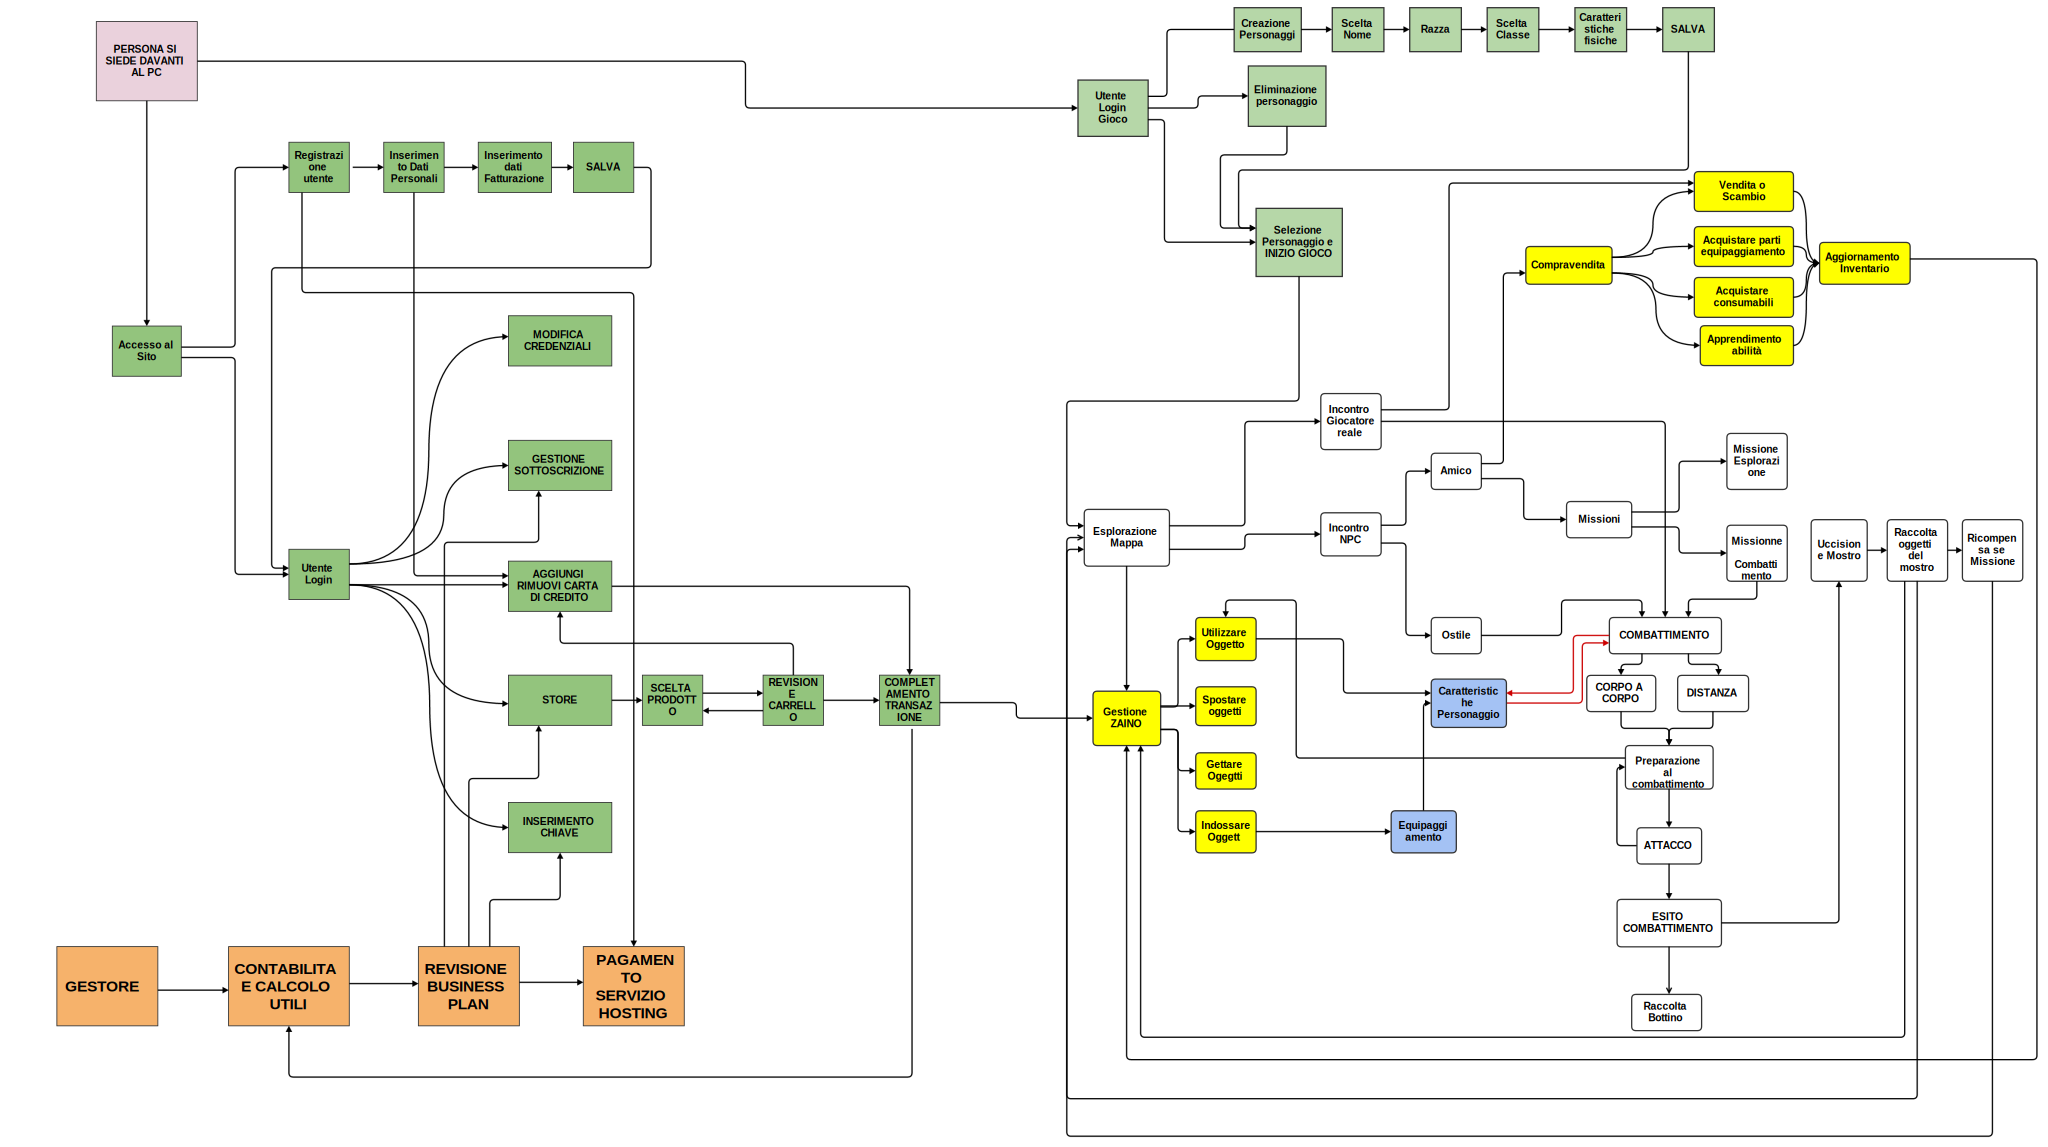
\includepdf[width=270mm, height=210mm, angle=90, keepaspectratio]{./pdf/sprocint.pdf}

\end{landscape}

 